\chapter{Bối cảnh bài toán: Quản lý Ngữ cảnh UE và tính dự đoán được\label{chapter:context}}
\chaptermark{Bối cảnh bài toán}

\section{Phân hệ Quản lý Ngữ cảnh UE}\label{sec:uecm}
Phân hệ được nghiên cứu là một dịch vụ Quản lý Ngữ cảnh UE. Dịch vụ này được mô hình hoá theo
một miền dịch vụ gNB-CU-CP thực tế của Nokia, sở hữu vòng đời ngữ cảnh UE, thực thi thủ tục
RRC~\cite{3gpp38331}, và di động/bàn giao, tức các chức năng mà kiến trúc 3GPP giao cho phần
mặt điều khiển của một gNB phân tách (Mục~\ref{sec:ranarch}).

Hình~\ref{fig:fsm} cho thấy máy trạng thái vòng đời ngữ cảnh UE mà cả hai bản hiện thực mã hoá
giống hệt nhau. Máy trạng thái này chính là thứ mà khối lượng công việc hỗn hợp ở
Mục~\ref{sec:workload} đưa mỗi UE đi qua.

\begin{figure}[ht]
\centering
\begin{tikzpicture}[
    ->, >=Stealth, node distance=3.2cm, font=\small,
    every state/.style={draw, minimum size=1.5cm, fill=blue!6, thick},
    every edge/.style={draw, thick}
  ]
  \node[state, initial, initial text=\scriptsize create] (idle) {Idle};
  \node[state, right=of idle] (conn) {Connected};
  \node[state, right=of conn] (reconf) {Reconf.};
  \node[state, below=1.9cm of conn, fill=gray!10] (rel) {Released};

  \path (idle)  edge node[above,font=\scriptsize]{setup} (conn)
        (conn)  edge[bend left=18] node[above,font=\scriptsize]{begin} (reconf)
        (reconf) edge[bend left=18] node[below,font=\scriptsize]{complete / abort} (conn)
        (conn)  edge node[right,font=\scriptsize,pos=0.45]{release} (rel)
        (idle)  edge[bend right=32] node[below,font=\scriptsize,pos=0.6]{release} (rel);
  \path (conn) edge[loop above] node[font=\scriptsize]{signal / add\_drb} (conn);
\end{tikzpicture}
\caption[Máy trạng thái vòng đời ngữ cảnh UE]{Máy trạng thái vòng đời ngữ cảnh UE. \texttt{create} cấp phát một ngữ cảnh ở
\texttt{Idle} và \texttt{setup} kết nối nó. \texttt{signal} và \texttt{add\_drb} được xử lý tại
chỗ khi ở \texttt{Connected}. Một tái cấu hình hoặc bàn giao đi qua \texttt{Reconfiguring} rồi
trở lại khi \texttt{complete} hoặc \texttt{abort}, còn \texttt{release} tháo dỡ ngữ cảnh. Thao
tác không hợp lệ với trạng thái hiện tại trả về \texttt{OpError} thay vì đổi trạng thái.\label{fig:fsm}}
\end{figure}

\paragraph{Vì sao chọn phân hệ này.}
UECM phù hợp làm đối tượng nghiên cứu vì vừa đại diện vừa đủ nhỏ để kiểm soát. Đây là chức năng
lớp~3 RAN cốt lõi, và mang các thuộc tính khiến mã mặt điều khiển sản xuất khó xử lý: trạng thái
có thể thay đổi theo từng UE, vòng đời thao tác chặt chẽ, mức độ đồng thời cao giữa các UE, cùng
mục tiêu độ trễ và độ tin cậy mà hệ thống 5G đặt ra cho thủ tục mặt điều
khiển~\cite{3gpp38913,3gpp22261}. Kết luận về cách một ngôn ngữ xử lý các thuộc tính đó do đó
chuyển được sang các dịch vụ mặt điều khiển có trạng thái và đồng thời khác. Phân hệ cũng đủ
nhỏ để đặc tả chính xác, hiện thực trung thực bằng hai ngôn ngữ, và suy luận trọn vẹn, tức điều
kiện tiên quyết để so sánh có kiểm thử tương đương trở nên khả thi. Một phân hệ lớn hơn sẽ đổi
lấy tính ngoại hiệu bằng tính nội hiệu mà một so sánh ngôn ngữ công bằng phụ thuộc vào. UECM
nằm ở điểm cả hai vẫn trong tầm với.

\paragraph{Tập thao tác.}
Giao diện mà nghiên cứu khai thác cố ý nhỏ và theo hướng vòng đời. Nó có thể tạo và giải phóng
một ngữ cảnh, thiết lập kết nối (\texttt{Idle}$\rightarrow$\texttt{Connected}), xử lý một thông
điệp báo hiệu trong phiên, thêm một data radio bearer, bắt đầu, hoàn tất hoặc huỷ một tái cấu
hình hoặc bàn giao, và tra cứu trạng thái ngữ cảnh dưới tải đồng thời. Mỗi thao tác được định
nghĩa cho mọi trạng thái của máy ở Hình~\ref{fig:fsm}: thao tác bất hợp pháp ở trạng thái hiện
tại trả về lỗi có kiểu và giữ nguyên ngữ cảnh, thay vì ném ngoại lệ hoặc làm hỏng trạng thái.
Tập thao tác kín và có kiểu này là điều cho phép cùng một bộ vectơ kiểm thử và cùng khối lượng
công việc dẫn cả hai bản hiện thực theo các đường đi giống hệt nhau (Mục~\ref{sec:parity}).

\section{Các lớp lỗi an toàn bộ nhớ và đồng thời}\label{sec:defects}
Các lỗi ảnh hưởng tới mã mặt điều khiển C++ loại này chia thành hai họ. Họ \emph{an toàn bộ
nhớ} liên quan tới vòng đời và biên của đối tượng: \emph{use-after-free} truy cập vùng nhớ đã
được giải phóng, \emph{double-free} giải phóng cùng một vùng hai lần, và \emph{buffer overflow}
đọc hoặc ghi vượt cuối vùng cấp phát. Họ \emph{đồng thời} liên quan tới truy cập không đồng bộ
hoặc sai thứ tự từ nhiều luồng: \emph{data race} là một cặp truy cập không đồng bộ vào cùng vị
trí mà ít nhất một bên là ghi, \emph{deadlock} là chờ khoá vòng, còn \emph{iterator invalidation}
là dùng iterator hoặc tham chiếu vào container sau khi một thay đổi đã di chuyển hoặc giải phóng
vùng nhớ bên dưới. Điểm chung là trong C++ chúng đều \emph{im lặng}: trình biên dịch chấp nhận
từng lớp, và trên các đường đi mà kiểm thử thông thường tình cờ chạm tới, chúng có thể trông
như hoạt động đúng, chỉ lộ ra sau dưới dạng hỏng dữ liệu, sập chương trình, hoặc đột biến độ trễ
không dự đoán được. Đây là cùng các lớp hỏng bộ nhớ mà hàng thập kỷ nghiên cứu bảo mật vẫn khó
kìm hãm trong C và C++~\cite{szekeres2013sok}.

Mỗi lớp có một hiện thân tự nhiên trong Quản lý Ngữ cảnh UE, đó là lý do phân hệ phù hợp để
nghiên cứu chúng:

\begin{itemize}
  \item \textbf{Use-after-free.} Một thông điệp báo hiệu giữ con trỏ thô hoặc tham chiếu tới
        ngữ cảnh UE mà một \texttt{release} đồng thời đã xoá khỏi bản đồ ngữ cảnh. Bộ xử lý
        đang bay khi đó giải tham chiếu vùng nhớ đã giải phóng.
  \item \textbf{Double-free.} Đường \texttt{release} chạy hai lần cho cùng một UE, ví dụ vì
        \texttt{release} được truyền lại không được làm bất biến, giải phóng tài nguyên sở hữu
        của ngữ cảnh lần thứ hai.
  \item \textbf{Iterator invalidation.} Mã lặp danh sách data radio bearer của ngữ cảnh trong khi
        thêm hoặc gỡ bearer, nên iterator trỏ vào vùng nhớ mà container đã tái cấp phát.
  \item \textbf{Data race.} Hai worker cập nhật cùng một trường ngữ cảnh, bộ đếm hoạt động hoặc
        cờ trạng thái, mà không đồng bộ hoá, nên các truy cập tranh chấp.
  \item \textbf{Unguarded shared mutation.} Một ngữ cảnh được chia sẻ bằng tham chiếu giữa các
        luồng và bị thay đổi mà không có khoá hay kỷ luật khác, một race mà nguyên nhân gốc là
        không có quy tắc sở hữu cho trạng thái dùng chung.
  \item \textbf{Use-after-move.} Thủ tục nhận di chuyển ngữ cảnh vừa dựng vào kho và rồi trả lời
        yêu cầu từ biến cục bộ vừa bị move khỏi, nên phản hồi mang danh tính rỗng. Lớp này được
        giữ vì công cụ C++ \emph{không} nói gì về nó. Không có gì bị hỏng và không có hành vi
        không xác định, vì đối tượng đã move vẫn ở trạng thái hợp lệ nhưng không xác định, nên
        lỗi không có triệu chứng lúc chạy để sanitiser bắt.
  \item \textbf{Thread-unsafe handle shared across workers.} Tay cầm ngữ cảnh đếm tham chiếu mà
        bộ đếm không nguyên tử, thói quen đường nóng chọn khi khối điều khiển nguyên tử của con
        trỏ chia sẻ tốn hơn lợi ích, được truyền cho hai shard worker. Ràng buộc khiến tay cầm
        đúng được viết trong comment, vì C++ không có cách diễn đạt gắn kết luồng trong kiểu.
\end{itemize}

Bảy lớp này nằm gọn trong các bảo đảm mà Rust tuyên bố, nên chúng là thử nghiệm tự nhiên xem
tuyên bố đó có đứng không. Tuy nhiên chỉ kiểm thử chúng sẽ khắc sẵn câu trả lời mong đợi vào
lựa chọn ca kiểm thử, nên thêm bảy lớp nữa được đưa vào nghiên cứu vì lý do ngược lại, tức có cơ
sở kỳ vọng Rust an toàn \emph{không} ngăn được chúng:

\begin{itemize}
  \item \textbf{Lock-order deadlock.} Một bàn giao khoá ngữ cảnh UE nguồn rồi đích, trong khi
        bàn giao đồng thời chiều ngược khoá đích rồi nguồn, và hai bên chờ nhau vô hạn. Không có
        gì vi phạm vòng đời đối tượng hay aliasing. Lỗi nằm ở thứ tự lấy khoá.
  \item \textbf{Lost update.} Hai worker tăng bộ đếm hoạt động của ngữ cảnh qua read-modify-write
        tách thành hai vùng tới hạn riêng. Mỗi truy cập riêng lẻ đều đồng bộ đúng, nên đây là
        \emph{race condition} chứ không phải \emph{data race}: vi phạm nguyên tử nằm ở tổ hợp
        thao tác, không phải ở bản thân truy cập bộ nhớ, và nó làm hỏng giá trị im lặng thay vì
        sập chương trình.
  \item \textbf{Leak through a reference cycle.} Một ngữ cảnh và đối tác bàn giao giữ tham chiếu
        sở hữu lẫn nhau, nên không bộ đếm nào về không và không bên nào bị huỷ. Đếm tham chiếu
        không thu gom chu trình trong cả hai ngôn ngữ, và rò rỉ là an toàn trong Rust theo thiết
        kế tường minh. Đây là phát biểu ranh giới rõ nhất trong danh mục, vì cả hai ngôn ngữ
        thất bại giống nhau.
  \item \textbf{Integer overflow in a release build.} Tính bước TEID của bearer vượt độ rộng
        kiểu. Trong C++ tràn số có dấu là \emph{không xác định}, nên chương trình không có
        nghĩa. Trong Rust nó \emph{được định nghĩa} là quấn vòng, vì hồ sơ \texttt{opt-level~=~2}
        mà nghiên cứu so sánh tắt \texttt{overflow-checks}, nên chương trình có nghĩa và nghĩa
        đó sai. Mẫu không giả định: CVE-2026-64467 trong \texttt{rust\_binder} là lỗi bước cùng
        hình dạng.
  \item \textbf{Worker failure blast radius.} Một shard worker thất bại giữa chừng thủ tục. Mô hình
        đồng thời ở Mục~\ref{sec:concurrency} biến một shard thành miền lỗi theo cấu trúc, và
        không hệ kiểu nào của hai ngôn ngữ buộc nó hành xử như vậy: trong C++ ngoại lệ thoát khỏi
        callable của luồng chấm dứt cả tiến trình, còn trong Rust panic giam trong luồng nhưng
        độc trạng thái nó giữ, nên thiệt hại lan theo dữ liệu. Trực tiếp liên quan tới luận điểm
        tính sẵn sàng cấp nhà mạng, và không gì trong hai hệ kiểu giải quyết.
  \item \textbf{Double-free across the seam.} Máy chủ C++ giữ tay cầm mờ tới ngữ cảnh Rust và
        giải phóng hai lần, tức \texttt{release} truyền lại của lớp double-free ở trên, giờ diễn
        đạt theo cách ranh giới hàm ngoại bắt buộc. Rust an toàn từ chối giải phóng kép vì sở
        hữu theo dõi giá trị. Một đường nối không giữ được điều đó, vì đưa con trỏ thô cho caller
        C chính là thao tác chấm dứt kiến thức của trình biên dịch về nó. Lớp do đó xuất hiện
        hai phía ranh giới, là phát biểu sắc nhất về bản chất ranh giới.
  \item \textbf{Forgotten lock guard.} Thiết lập bearer lấy khoá ngữ cảnh và lỗi kiểm tra khiến
        hàm trả về mà không nhả khoá, nên worker kế tiếp chạm ngữ cảnh đó chờ vô hạn. Rust loại
        dạng thường gặp của lỗi này, vì guard nhả khi bị drop và không có unlock viết tay để bỏ
        qua. Nó không loại bỏ lỗi, vì guard là một giá trị và rò rỉ giá trị là an toàn. Nơi chu
        trình tham chiếu rò bộ nhớ, đây rò chính ngữ cảnh.
\end{itemize}

Cùng nhau mười bốn lớp này tạo danh mục được tiêm ở Chương~\ref{chapter:eval}, và sự tách hai
nhóm là điều cho phép nghiên cứu báo cáo một ranh giới thay vì một phán quyết. Buffer overflow
được mô tả ở trên cho đầy đủ nhưng không được tiêm, vì không bản hiện thực nào làm số học con trỏ
thô trên kho ngữ cảnh, nên một ca tiêm sẽ là cấu trúc giả tạo chứ không phải lỗi hợp lý trong
phân hệ này. Bảng~\ref{tab:defectmap} gom danh mục với kết quả kỳ vọng của từng ca \emph{trước}
khi nghiên cứu chạy, đúng dạng mà runner ghi nhận: một kỳ vọng viết trước có thể bị vi phạm theo
cả hai chiều và được báo là sai lệch, còn kỳ vọng hình thành sau sự kiện thì không thể.

\begin{table}[H]
\centering
\small
\caption[Danh mục tiêm và hiện thân trong UECM]{Danh mục lỗi tiêm: mỗi lớp theo hình thức hợp lý trong Quản lý Ngữ cảnh UE, và
kết quả ghi nhận trước nghiên cứu. Cột cuối là dự đoán chứ không phải kết quả. Bảng~\ref{tab:taxonomy}
báo cáo điều đã đo, và runner lỗi đánh dấu sai khác theo cả hai chiều thay vì hấp thụ vào kết
luận. Buffer overflow được liệt kê cho đầy đủ và không tiêm: không bản hiện thực nào làm số học
con trỏ trên kho ngữ cảnh.\label{tab:defectmap}}
\footnotesize
\renewcommand{\arraystretch}{0.95}
\begin{tabular}{@{}R{0.19\linewidth} R{0.40\linewidth} R{0.14\linewidth} R{0.16\linewidth}@{}}
\hline\hline
Lớp lỗi & Hiện thân trong Quản lý Ngữ cảnh UE & Cách thất bại & Kỳ vọng trong Rust an toàn \\
\hline
\multicolumn{4}{@{}l}{\emph{Họ an toàn bộ nhớ: vòng đời và biên đối tượng}} \\
Use-after-free & Bộ xử lý báo hiệu đang bay giải tham chiếu ngữ cảnh mà \texttt{release} đồng thời đã xoá khỏi bản đồ & Hỏng dữ liệu hoặc sập & Ngăn chặn \\
Double-free & \texttt{release} truyền lại không bất biến, nên đường giải phóng giải phóng tài nguyên ngữ cảnh lần hai & Hỏng dữ liệu hoặc sập & Ngăn chặn \\
Use-after-move & Thủ tục nhận trả lời từ ngữ cảnh vừa move vào kho & Danh tính rỗng im lặng & Ngăn chặn \\
Buffer overflow & Không có hiện thân hợp lý: kho ngữ cảnh chỉ qua API container & n/a & Không tiêm \\
\hline
\multicolumn{4}{@{}l}{\emph{Họ đồng thời: truy cập không đồng bộ hoặc sai thứ tự}} \\
Iterator invalidation & Bearer được thêm trong khi đang lặp danh sách data radio bearer của ngữ cảnh & Hỏng dữ liệu hoặc sập & Ngăn chặn \\
Data race & Hai worker cập nhật cùng trường ngữ cảnh, bộ đếm hoặc cờ trạng thái, không đồng bộ & Giá trị xé hoặc mất & Ngăn chặn \\
Unguarded shared mutation & Ngữ cảnh chia sẻ giữa luồng và bị thay đổi không có quy tắc sở hữu & Giá trị xé hoặc mất & Ngăn chặn \\
Thread-unsafe handle shared & Tay cầm ngữ cảnh có bộ đếm không nguyên tử được truyền cho hai shard worker & Bộ đếm hỏng & Ngăn chặn \\
\hline
\multicolumn{4}{@{}l}{\emph{Nhóm ranh giới: đưa vào vì Rust an toàn được kỳ vọng \emph{không} ngăn chúng}} \\
Lock-order deadlock & Hai bàn giao đối chiều khoá nguồn-rồi-đích và đích-rồi-nguồn & Treo & Không ngăn \\
Lost update & Read-modify-write của bộ đếm tách qua hai vùng tới hạn, mỗi truy cập đồng bộ nhưng tổ hợp không nguyên tử & Giá trị sai im lặng & Không ngăn \\
Reference-cycle leak & Ngữ cảnh và đối tác bàn giao giữ tham chiếu sở hữu lẫn nhau, nên không bộ đếm nào về không & Tăng trưởng không giới hạn & Không ngăn \\
Integer overflow (release build) & Tính bước TEID của bearer vượt độ rộng kiểu & Giá trị sai im lặng & Không ngăn \\
Worker-failure blast radius & Một shard worker thất bại giữa thủ tục khi đang giữ trạng thái shard & Sự cố vượt một shard & Không ngăn \\
Double-free across the seam & Máy chủ C++ giải phóng tay cầm mờ tới ngữ cảnh Rust hai lần & Hỏng dữ liệu hoặc sập & Không ngăn \\
Forgotten lock guard & Thiết lập bearer trả về khi kiểm tra thất bại mà không nhả khoá ngữ cảnh & Treo & Không ngăn \\
\hline
\end{tabular}
\end{table}

\section{Độ trễ đuôi và tính dự đoán được trong RAN}
Mục~\ref{sec:predictability} đã nêu vì sao đuôi chứ không phải trung vị chi phối hệ nhạy độ trễ,
và đo đúng đòi hỏi gì. Điều mục đó để ở mức chung, mục này làm cụ thể, vì hai thuộc tính của bối
cảnh RAN biến ưu tiên phương pháp thành chỉ số chi phối.

Hai thuộc tính đó là fan-out và quy mô, minh hoạ ở Hình~\ref{fig:tailconcept}. Một hành động
người dùng thấy, thiết lập cuộc gọi hoặc bàn giao, trở thành nhiều thao tác mặt điều khiển phụ
thuộc mà thành phần chậm nhất chặn hoàn tất, và một trạm bận đẩy hàng nghìn thủ tục như vậy mỗi
giây trên hàng triệu thiết bị kết nối. Gộp lại, p99.9 của một thao tác Quản lý Ngữ cảnh UE không
phải nét lạ ở rìa phân phối. Đó là tốc độ thủ tục suy giảm mà mạng duy trì liên tục.

Quy mô mà các phân vị đó quan trọng không phải giả định. Một nghiên cứu đo trên RAN 5G phân tách
đo thủ tục UE Context Setup từ CU-CP tới DU qua F1-C, và thiết lập ngữ cảnh bearer từ CU-CP tới
CU-UP qua E1, dưới các sơ đồ bảo vệ giao diện khác nhau, và thấy lựa chọn đáng hàng trăm micro
giây: trên F1-C, IPsec thêm cỡ $120\,\mu$s trung bình cho thiết lập ngữ cảnh UE, so với khoảng
$430\,\mu$s cho DTLS~\cite{michaelides2026ranlatency}. Chi phí cỡ đó được coi là đáng kể đúng với
họ thủ tục mà luận văn tái hiện thực, điều đặt các thao tác này vào chế độ mà hàng chục micro giây
là đại lượng kỹ thuật chứ không phải nhiễu.

Nghiên cứu do đó đặc trưng hoá toàn bộ phân phối độ trễ, tập trung vào các phân vị cao (p99 và
p99.9) và giá trị cực đại, cùng cách chúng suy giảm khi tải đưa vào tiến tới rồi vượt bão hoà
(Chương~\ref{chapter:eval}). Dừng ở tải danh định sẽ bỏ lỡ chế độ quyết định chất lượng dịch vụ,
vì độ trễ xếp hàng tăng siêu tuyến gần công suất. Đó cũng là chế độ mà khác biệt giữa hai bản
hiện thực của một thiết kế, nếu có, còn chỗ để lộ ra.

\begin{figure}[ht]
\centering
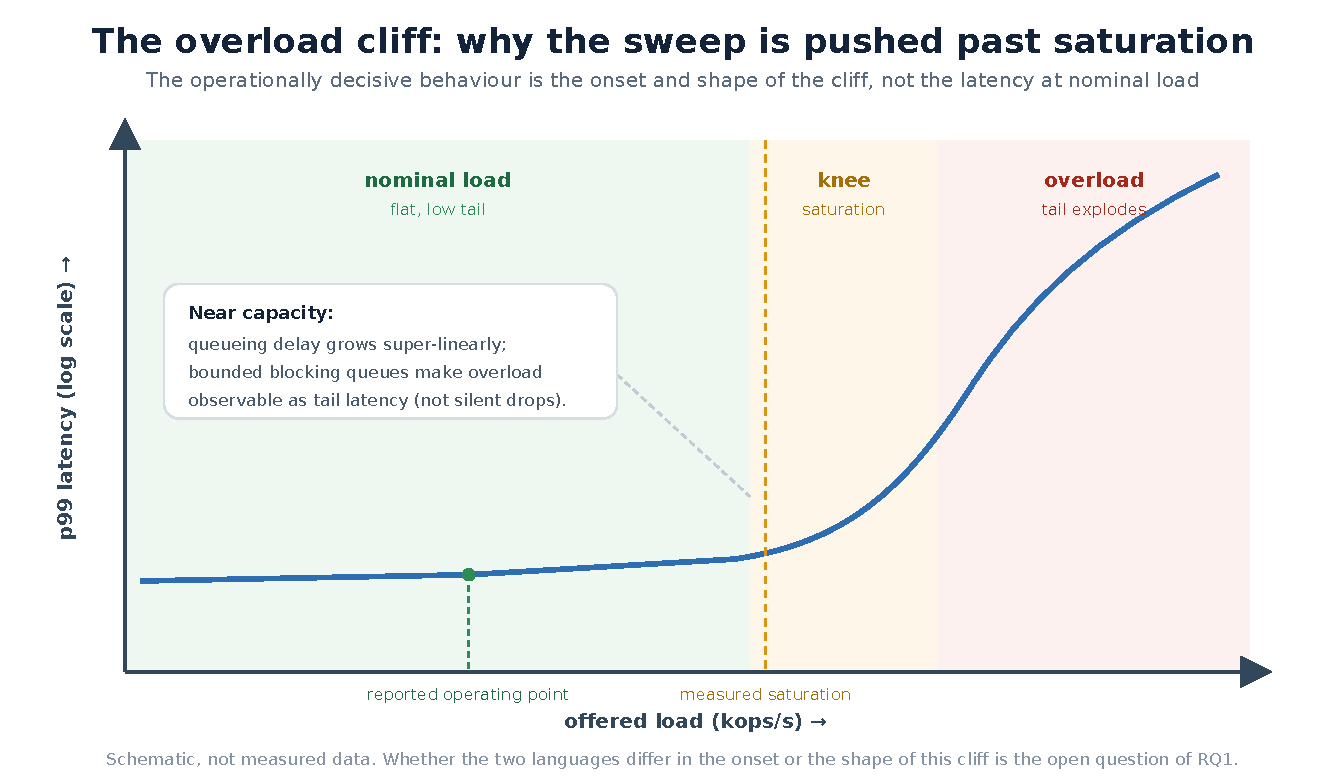
\includegraphics[width=0.70\linewidth]{diagrams/pdf/15_overload_cliff.pdf}
\caption[Vách quá tải]{Vách quá tải. Độ trễ đuôi thấp và phẳng khi tải đưa vào dưới công suất phục vụ, rồi
leo dốc mạnh khi hệ thống bị đẩy qua bão hoà và yêu cầu xếp hàng sau các hàng đợi chặn có giới
hạn. Hành vi quyết định vận hành là chỗ và hình dạng vách này bắt đầu, đó là lý do quét tải được
đẩy qua điểm bão hoà thay vì dừng ở tải danh định. Hình là sơ đồ hiện tượng chứ không phải đồ
thị dữ liệu nghiên cứu: liệu hai ngôn ngữ có khác ở chỗ vách bắt đầu hay độ dốc leo chính là điều
RQ1 hỏi, và Mục~\ref{sec:perfresults} báo cáo máy phát triển không phân giải được.\label{fig:cliff}}
\end{figure}
